\documentclass[12pt,a4paper]{paper}
\usepackage[utf8]{inputenc}
\usepackage[english]{babel}
\usepackage{amsmath}
\usepackage{enumitem}
\usepackage{fixltx2e}
\usepackage{multicol}
\usepackage{amsmath}
\usepackage{enumitem}
\usepackage{arydshln}
\usepackage{amsfonts}
\usepackage{multirow}
\usepackage{multicol}
\usepackage{amssymb}
\usepackage{amsfonts}
\usepackage{amssymb}
\usepackage[left=1cm,right=1cm,top=1.5cm,bottom=2cm]{geometry}
\usepackage{Sweave}
\begin{document}
\title{STAT636 - Homework 6\\\small{Daniel Osorio - dcosorioh@tamu.edu\\Department of Veterinary Integrative Biosciences\\Texas A\&M University}}
\maketitle
\Sconcordance{concordance:HW6_DanielOsorio.tex:HW6_DanielOsorio.Rnw:%
1 17 1 1 0 5 1 1 2 1 0 2 1 3 0 1 2 3 1 1 2 1 0 3 1 25 0 2 2 4 0 2 2 1 0 %
2 1 23 0 8 1 1 3 2 0 2 1 4 0 1 2 4 1 1 2 1 0 3 1 26 0 6 1 1 3 2 0 2 1 4 %
0 2 2 1 0 2 1 24 0 4 1 1 4 3 0 2 1 4 0 1 2 1 1 1 2 1 0 1 3 2 0 1 1 12 0 %
1 1 1 3 2 0 1 1 4 0 1 2 2 1 1 2 4 0 1 2 1 1 1 2 1 0 3 1 4 0 1 2 1 1 1 2 %
7 0 1 2 1 1 1 2 1 0 8 1 6 0 1 2 2 1 1 2 1 0 1 1 3 0 1 2 1 1 1 2 14 0 2 %
2 1 0 1 1 4 0 1 2 1 1 1 2 1 0 1 5 4 0 1 1 6 0 1 2 4 1 1 4 3 0 6 1 3 0 1 %
2 1 1 1 3 2 0 1 1 8 0 1 2 6 0 1 2 6 0 1 2 7 0 2 2 1 0 1 3 2 0 1 6 5 0 1 %
1 1 2 5 0 1 2 1 1 1 8 7 0 1 1 6 0 1 1 6 0 1 2 2 1 1 2 1 0 1 2 1 0 1 1 1 %
16 15 0 1 5 8 0 1 2 3 1}

\begin{enumerate}
\item Consider the \texttt{Life\_Expectancy} data. Let the response $Y$ be \texttt{Life.expectancy}, and consider the numeric variables \texttt{Income.composition.of.resources}, and \texttt{Schooling} as the predictor variables. For the purpose of predicting the value of $Y$ , we will consider non-linear models.
\begin{Schunk}
\begin{Sinput}
> lifeExpectancy <- read.csv("Life_Expectancy.csv")
> lifeExpectancy <- lifeExpectancy[,c("Life.expectancy","Schooling")]
> lifeExpectancy <- lifeExpectancy[complete.cases(lifeExpectancy),]
\end{Sinput}
\end{Schunk}
\begin{enumerate}
\item Polynomial regression.
\begin{enumerate}
\item First predict \texttt{Life.expectancy} using a fourth-degree polynomial in \texttt{Schooling}. From the p-value of coefficients, what degree of polynomial do you think is necessary? \textit{From the p-values, less than 4.}
\begin{Schunk}
\begin{Sinput}
> lifeExpectancy[,2:5] <- sapply(1:4, function(x){lifeExpectancy[,2]^x})
> colnames(lifeExpectancy) <- c("Y", "X1", "X2", "X3", "X4")
> p4 <- lm(Y~., data = lifeExpectancy[,1:5])
> summary(p4)
\end{Sinput}
\begin{Soutput}
Call:
lm(formula = Y ~ ., data = lifeExpectancy[, 1:5])

Residuals:
     Min       1Q   Median       3Q      Max 
-16.6941  -2.3720   0.7387   3.2998  14.2940 

Coefficients:
              Estimate Std. Error t value Pr(>|t|)    
(Intercept) 61.2162412  9.8500202   6.215 3.92e-09 ***
X1          -3.0767145  4.4020089  -0.699    0.486    
X2           0.3793709  0.6931948   0.547    0.585    
X3          -0.0004507  0.0449784  -0.010    0.992    
X4          -0.0004257  0.0010250  -0.415    0.678    
---
Signif. codes:  0 ‘***’ 0.001 ‘**’ 0.01 ‘*’ 0.05 ‘.’ 0.1 ‘ ’ 1

Residual standard error: 5.339 on 168 degrees of freedom
Multiple R-squared:  0.6578,	Adjusted R-squared:  0.6496 
F-statistic: 80.73 on 4 and 168 DF,  p-value: < 2.2e-16
\end{Soutput}
\end{Schunk}
\item Use a third-degree polynomial in \texttt{Schooling} to fit the data again. Then create a grid of values for \texttt{Schooling}
\begin{Schunk}
\begin{Sinput}
> school_grid <- seq(from = 1.53, to = 20.04)
\end{Sinput}
\end{Schunk}
and make predictions for each. Finally plot the data, and add the fit from the degree-3 polynomial, with 2 times the standard error shown as error bars.
\begin{Schunk}
\begin{Sinput}
> lifeExpectancy <- lifeExpectancy[,1:4]
> p3 <- lm(Y~., data = lifeExpectancy)
> summary(p3)
\end{Sinput}
\begin{Soutput}
Call:
lm(formula = Y ~ ., data = lifeExpectancy)

Residuals:
     Min       1Q   Median       3Q      Max 
-16.8110  -2.2120   0.7029   3.2088  14.2981 

Coefficients:
             Estimate Std. Error t value Pr(>|t|)    
(Intercept) 64.183066   6.764306   9.488  < 2e-16 ***
X1          -4.711970   1.962702  -2.401 0.017447 *  
X2           0.656973   0.182969   3.591 0.000432 ***
X3          -0.018992   0.005419  -3.505 0.000585 ***
---
Signif. codes:  0 ‘***’ 0.001 ‘**’ 0.01 ‘*’ 0.05 ‘.’ 0.1 ‘ ’ 1

Residual standard error: 5.326 on 169 degrees of freedom
Multiple R-squared:  0.6574,	Adjusted R-squared:  0.6513 
F-statistic: 108.1 on 3 and 169 DF,  p-value: < 2.2e-16
\end{Soutput}
\begin{Sinput}
> school_grid <- as.data.frame(sapply(1:3, function(x){school_grid^x}))
> colnames(school_grid) <- c("X1", "X2", "X3")
> sE <- predict(p3,school_grid, se.fit = TRUE)
> par(mar=c(4,4,1,1), mgp = c(1.7,0.5,0))
> x <- school_grid[,1]
> ubSE <- sE$fit + (2* sE$se.fit)
> lbSE <- sE$fit - (2* sE$se.fit)
> yLim <- c(lbSE, ubSE)
> plot(lifeExpectancy[,2:1], 
+      pch = 20, col = "gray80", las = 1, xlab= "Schooling", 
+      ylab= "Life Expectancy", ylim= c(min(yLim), max(yLim)))
> points(y = sE$fit, x = x, type = "l" ,col= "red", lwd=2)
> arrows(x,ubSE,x,lbSE, length=0.05, angle=90, code=3, col = "red")
\end{Sinput}
\end{Schunk}
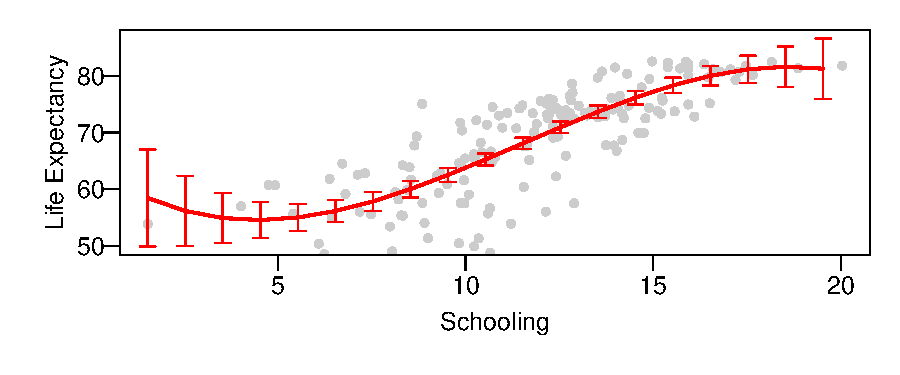
\includegraphics{HW6_DanielOsorio-004}
\end{enumerate}
\item Splines.
\begin{enumerate}
\item Fit \texttt{Life.expectancy} to \texttt{Schooling} using a regression model with cubic splines with specified knots at \texttt{Schooling} 5, 10 and 15. Make predictions at the grid you created above, and plot the data and add your cubic splines with 2 times the standard error
shown as error bars.
\begin{Schunk}
\begin{Sinput}
> library(splines)
> lifeExpectancy <- lifeExpectancy[,1:2]
> b1 <- lm(Y ~ bs(X1, knots = c(5,10,15)), data = lifeExpectancy)
> summary(b1)
\end{Sinput}
\begin{Soutput}
Call:
lm(formula = Y ~ bs(X1, knots = c(5, 10, 15)), data = lifeExpectancy)

Residuals:
     Min       1Q   Median       3Q      Max 
-16.6422  -2.1313   0.8818   3.1406  14.9636 

Coefficients:
                              Estimate Std. Error t value Pr(>|t|)    
(Intercept)                     53.809      5.317  10.120  < 2e-16 ***
bs(X1, knots = c(5, 10, 15))1   12.293     10.042   1.224 0.222623    
bs(X1, knots = c(5, 10, 15))2   -2.830      6.644  -0.426 0.670643    
bs(X1, knots = c(5, 10, 15))3    8.877      5.866   1.513 0.132146    
bs(X1, knots = c(5, 10, 15))4   26.251      5.916   4.438 1.65e-05 ***
bs(X1, knots = c(5, 10, 15))5   27.046      6.368   4.247 3.60e-05 ***
bs(X1, knots = c(5, 10, 15))6   28.522      7.219   3.951 0.000115 ***
---
Signif. codes:  0 ‘***’ 0.001 ‘**’ 0.01 ‘*’ 0.05 ‘.’ 0.1 ‘ ’ 1

Residual standard error: 5.318 on 166 degrees of freedom
Multiple R-squared:  0.6646,	Adjusted R-squared:  0.6525 
F-statistic: 54.82 on 6 and 166 DF,  p-value: < 2.2e-16
\end{Soutput}
\begin{Sinput}
> X1 <- school_grid[,1]
> sE <- predict(b1,bs(X1, knots = c(5,10,15)), se.fit = TRUE)
> x <- school_grid[,1]
> ubSE <- sE$fit + (2* sE$se.fit)
> lbSE <- sE$fit - (2* sE$se.fit)
> par(mar=c(4,4,1,1), mgp = c(1.7,0.5,0))
> plot(lifeExpectancy[,2:1], pch = 20, col = "gray80", las = 1, 
+      xlab= "Schooling", ylab= "Life Expectancy", 
+      ylim= c(min(c(lbSE, ubSE)), max(c(lbSE, ubSE))))
> points(y = sE$fit, x = x, type = "l" ,col= "red", lwd=2)
> arrows(x,ubSE,x,lbSE, length=0.05, angle=90, code=3, col = "red")
\end{Sinput}
\end{Schunk}
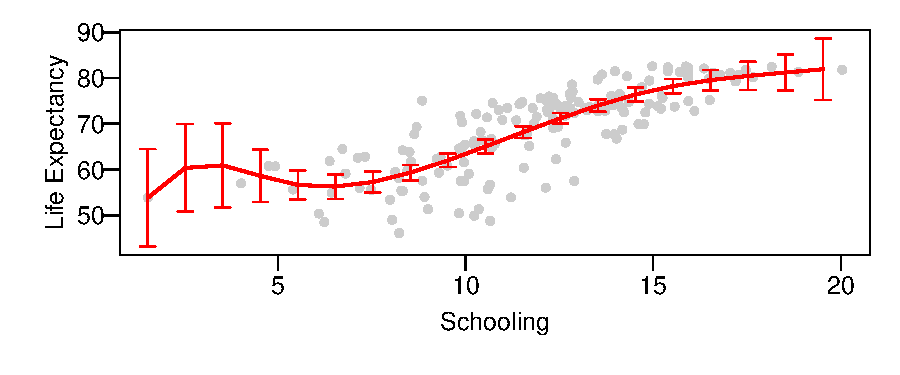
\includegraphics{HW6_DanielOsorio-005}
\item Fit \texttt{Life.expectancy} to \texttt{Schooling} using a regression model with nature splines with degree of freedom 4. Make predictions at the grid you created above, and plot the data and add your cubic splines with 2 times the standard error shown as error bars. Note that at the boundary of data, nature splines are better than basic cubic splines.
\begin{Schunk}
\begin{Sinput}
> library(splines)
> b2 <- lm(Y ~ ns(X1, df = 4), data = lifeExpectancy)
> summary(b2)
\end{Sinput}
\begin{Soutput}
Call:
lm(formula = Y ~ ns(X1, df = 4), data = lifeExpectancy)

Residuals:
     Min       1Q   Median       3Q      Max 
-16.5018  -2.2104   0.8687   3.2655  15.2364 

Coefficients:
                Estimate Std. Error t value Pr(>|t|)    
(Intercept)       58.039      3.789  15.316  < 2e-16 ***
ns(X1, df = 4)1   13.319      3.648   3.651 0.000348 ***
ns(X1, df = 4)2   21.800      2.728   7.991 2.04e-13 ***
ns(X1, df = 4)3   19.085      8.430   2.264 0.024847 *  
ns(X1, df = 4)4   28.507      3.715   7.673 1.30e-12 ***
---
Signif. codes:  0 ‘***’ 0.001 ‘**’ 0.01 ‘*’ 0.05 ‘.’ 0.1 ‘ ’ 1

Residual standard error: 5.267 on 168 degrees of freedom
Multiple R-squared:  0.6669,	Adjusted R-squared:  0.659 
F-statistic: 84.09 on 4 and 168 DF,  p-value: < 2.2e-16
\end{Soutput}
\begin{Sinput}
> sE <- predict(b2,ns(X1, df = 4), se.fit = TRUE)
> ubSE <- sE$fit + (2* sE$se.fit)
> lbSE <- sE$fit - (2* sE$se.fit)
> par(mar=c(4,4,1,1), mgp = c(1.7,0.5,0))
> plot(lifeExpectancy[,2:1], 
+      pch = 20, col = "gray80", 
+      las = 1, xlab= "Schooling", ylab= "Life Expectancy", 
+      ylim= c(min(c(lbSE, ubSE)), max(c(lbSE, ubSE))))
> points(y = sE$fit, x = x, type = "l" ,col= "red", lwd=2)
> arrows(x,ubSE,x,lbSE, length=0.05, angle=90, code=3, col = "red")
\end{Sinput}
\end{Schunk}
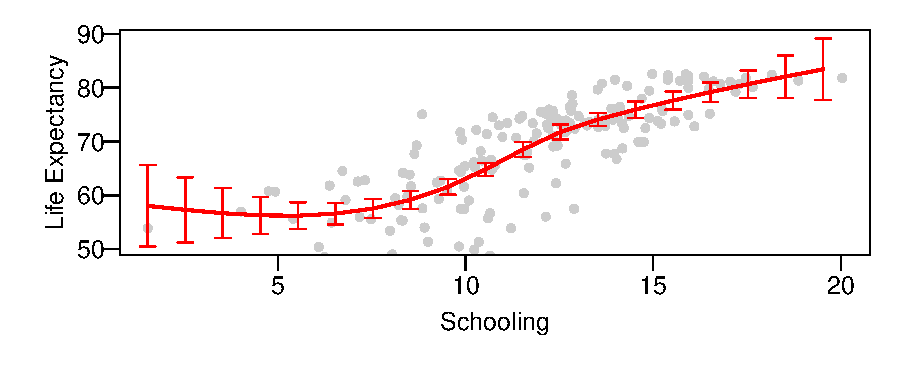
\includegraphics{HW6_DanielOsorio-006}
\item For smoothing splines, select the $\lambda$ by cross-validation; what's your result? Also
plot the data and add your smoothing splines.
\begin{Schunk}
\begin{Sinput}
> lifeExpectancy <- unique(lifeExpectancy)
> b3 <- smooth.spline(x = lifeExpectancy[,2], 
+                     y = lifeExpectancy[,1], 
+                     cv = TRUE)
> b3
\end{Sinput}
\begin{Soutput}
Call:
smooth.spline(x = lifeExpectancy[, 2], y = lifeExpectancy[, 1], 
    cv = TRUE)

Smoothing Parameter  spar= 1.072785  lambda= 0.004107205 (17 iterations)
Equivalent Degrees of Freedom (Df): 5.57255
Penalized Criterion (RSS): 4382.429
PRESS(l.o.o. CV): 28.2348
\end{Soutput}
\begin{Sinput}
> par(mar=c(4,4,1,1), mgp = c(1.7,0.5,0))
> plot(lifeExpectancy[,2:1], 
+      pch = 20, col = "gray80", las = 1, 
+      xlab= "Schooling", ylab= "Life Expectancy")
> points(x = b3$x, y = b3$y, type = "l", col = "red", lwd=2)
\end{Sinput}
\end{Schunk}
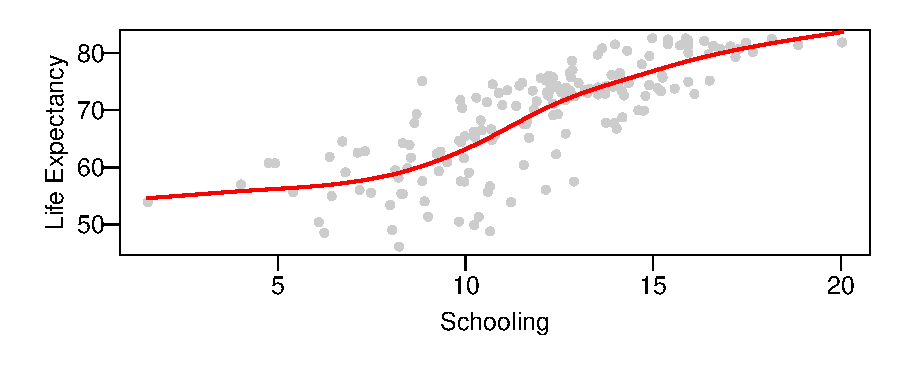
\includegraphics{HW6_DanielOsorio-007}
\end{enumerate}
\end{enumerate}
\item  Consider the \texttt{wine\_quality\_red data}. These contain eleven different variables (1 : fixed acidity; 2 : volatile acidity; 3 : citric acid; 4 : residual sugar; 5 : chlorides; 6 : free sulfur dioxide; 7 : total sulfur dioxide; 8 : density; 9 : pH; 10 : sulphates; 11 : alcohol) and one output (quality (score between 0 and 10) ). Use \texttt{tree} method and \texttt{random forest} method to perform classification.
\begin{Schunk}
\begin{Sinput}
> wineData <- read.csv("winequality_red.csv")
\end{Sinput}
\end{Schunk}
\begin{enumerate}
\item  Use tree method to do classification, and plot the tree graph
\begin{Schunk}
\begin{Sinput}
> treeModel <- tree::tree(quality~., wineData)
> par(mar=c(1,1,1,1))
> plot(treeModel)
> text(treeModel)
\end{Sinput}
\end{Schunk}
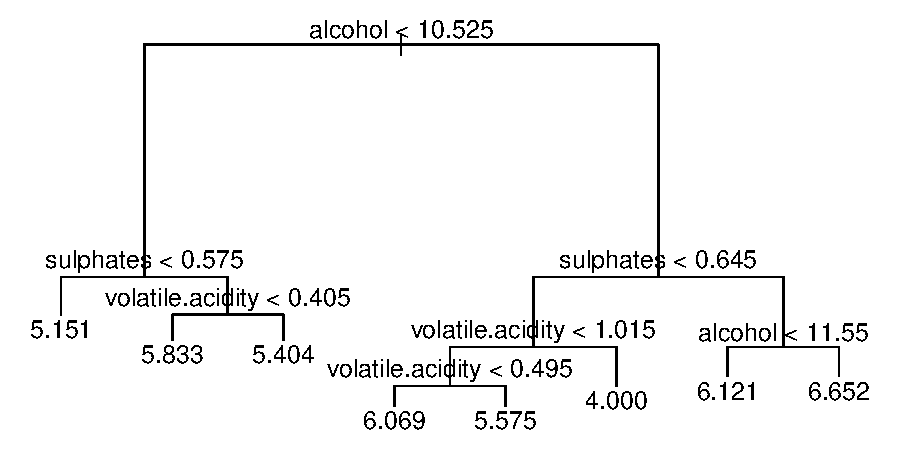
\includegraphics{HW6_DanielOsorio-009}
\begin{enumerate}
\item  What’s the training error rate?
\begin{Schunk}
\begin{Sinput}
> mean((wineData$quality - predict(treeModel))^2)
\end{Sinput}
\begin{Soutput}
[1] 0.4254908
\end{Soutput}
\end{Schunk}
\item  Randomly sample 1000 rows as training data and use tree method to do classification.
What’s the accuracy rate for test data? (Do \texttt{set.seed(1)} before sampling.)
\begin{Schunk}
\begin{Sinput}
> set.seed(1)
> n <- seq_len(nrow(wineData))
> training <- sample(n, size = 1000)
> testing <- n[!n %in% training]
> training <- wineData[training,]
> testing <- wineData[testing,]
> treeModel <- rpart::rpart(quality~., training)
> prediction <- predict(treeModel, newdata = testing[,-12])
> mean((testing$quality - prediction)^2)
\end{Sinput}
\begin{Soutput}
[1] 0.4353023
\end{Soutput}
\end{Schunk}
\end{enumerate}
\item Use a random forest to do classification with the same training data set. At each split,
allow 7 variables to be considered. (Do \texttt{set.seed(1)} before doing random forest.)
\begin{Schunk}
\begin{Sinput}
> set.seed(1)
> rForest <- randomForest::randomForest(quality~., training, mtry = 7)
\end{Sinput}
\end{Schunk}
\begin{enumerate}
\item What’s the accuracy rate now?
\begin{Schunk}
\begin{Sinput}
> rForest
\end{Sinput}
\begin{Soutput}
Call:
 randomForest(formula = quality ~ ., data = training, mtry = 7) 
               Type of random forest: regression
                     Number of trees: 500
No. of variables tried at each split: 7

          Mean of squared residuals: 0.3818267
                    % Var explained: 41.82
\end{Soutput}
\end{Schunk}
\item Use \texttt{varImpPlot} to plot the importance figure. What’s the most important factor? \textit{Alcohol}
\begin{Schunk}
\begin{Sinput}
> par(mar=c(4,4,1,1), mgp = c(1.7,0.5,0))
> randomForest::varImpPlot(rForest)
\end{Sinput}
\end{Schunk}
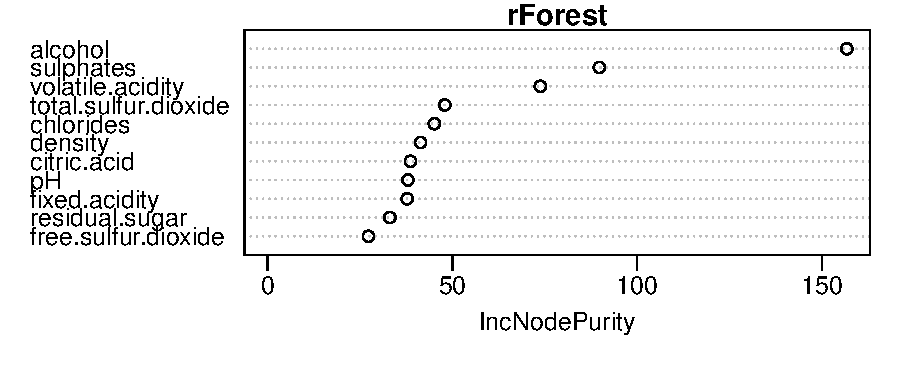
\includegraphics{HW6_DanielOsorio-014}
\item Use bootstrap (100 times) to estimate the standard deviation of classification accuracies.
(\texttt{set.seed(1)} before bootstrap)
\begin{Schunk}
\begin{Sinput}
> set.seed(1)
> MSE <- sapply(1:100, function(x){
+   selectedR <- sample(seq_len(nrow(testing)), replace = TRUE)
+   prediction <- predict(rForest,testing[selectedR, 1:11])
+   mean((testing[selectedR,12] - prediction)^2)
+ })
> sd(MSE)
\end{Sinput}
\begin{Soutput}
[1] 0.02706819
\end{Soutput}
\end{Schunk}
\end{enumerate}
\item Consider the binary classification problem. Suppose we denote the wine whose quality
is larger than 5 as `good', otherwise we think it is `bad'. Similarly as before, randomly
sample 1000 observations as training set, and use the tree method to do classification
again. (\texttt{set.seed(1)} before sampling)
\begin{Schunk}
\begin{Sinput}
> wineData[,12] <- factor(ifelse(test = wineData[,12] > 5, 
+                                yes = "G", 
+                                no = "B"))
> set.seed(1)
> training <- sample(n, size = 1000)
> testing <- n[!n %in% training]
> training <- wineData[training,]
> testing <- wineData[testing,]
> bC <- tree::tree(quality~., training)
\end{Sinput}
\end{Schunk}
\begin{enumerate}
\item What’s the accuracy rate, sensitivity and specificity?
\begin{Schunk}
\begin{Sinput}
> ConfussionMatrix <- table(Observed=testing[,12],
+   Predicted=predict(bC,testing[,-12], type = "class"))
> ConfussionMatrix
\end{Sinput}
\begin{Soutput}
        Predicted
Observed   B   G
       B 225  35
       G 127 212
\end{Soutput}
\begin{Sinput}
> # Accuracy
> sum(diag(ConfussionMatrix)/sum(ConfussionMatrix))
\end{Sinput}
\begin{Soutput}
[1] 0.7295492
\end{Soutput}
\begin{Sinput}
> # Sensitivity (True Positive Rate)
> ConfussionMatrix[2,2]/sum(ConfussionMatrix[2,])
\end{Sinput}
\begin{Soutput}
[1] 0.6253687
\end{Soutput}
\begin{Sinput}
> # Specificity (True Negative Rate)
> ConfussionMatrix[1,1]/sum(ConfussionMatrix[1,])
\end{Sinput}
\begin{Soutput}
[1] 0.8653846
\end{Soutput}
\end{Schunk}
\item Let $\kappa$\texttt{ = seq(from = 0, to = 1, by = 0.01)}. Plot the ROC curve.
\begin{Schunk}
\begin{Sinput}
> bProb <- predict(bC,testing[,-12])[,1]
> K <- sapply(seq(from = 0, to = 1, by = 0.01), function(x){
+   ifelse(test = bProb > x,yes = "B", no = "G")
+ })
> ROC <- t(apply(K,2,function(hat){
+   ConfussionMatrix <- table(Observed=testing[,12],
+                             Predicted=factor(hat, levels = c("B","G")))
+   c(ConfussionMatrix[1,2]/sum(ConfussionMatrix[1,]),
+     ConfussionMatrix[2,2]/sum(ConfussionMatrix[2,]))
+ }))
> par(mar=c(4,4,1,1), mgp=c(1.6,0.5,0))
> plot(ROC, type = "l", ylab = "True Positive Rate", 
+      xlab = "False Positive Rate", main = "ROC", las = 1)
\end{Sinput}
\end{Schunk}
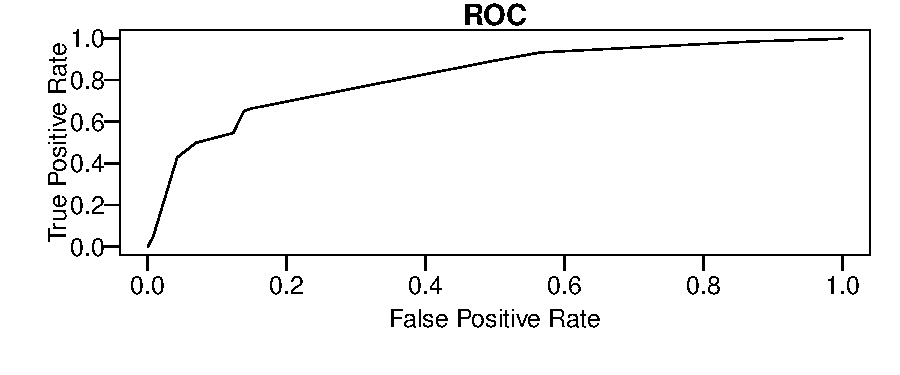
\includegraphics{HW6_DanielOsorio-018}
\item Use cross validation to decide the number of nodes. What’s the best choice?
(\texttt{set.seed(1)} before cross validation)
\begin{Schunk}
\begin{Sinput}
> accNodes <- c(NA,sapply(2:12, function(nNumber){
+   hat <- predict(tree::prune.tree(bC, best = nNumber),
+                  testing[,-12], "class")
+   ConfussionMatrix <- table(Observed=testing[,12],
+                             Predicted=factor(hat, levels = c("B","G")))
+   sum(diag(ConfussionMatrix)/sum(ConfussionMatrix))
+ }))
> accNodes
\end{Sinput}
\begin{Soutput}
 [1]        NA 0.7061770 0.7061770 0.7061770 0.7061770 0.7345576 0.7378965
 [8] 0.7378965 0.7445743 0.7312187 0.7312187 0.7295492
\end{Soutput}
\begin{Sinput}
> which.max(accNodes)
\end{Sinput}
\begin{Soutput}
[1] 9
\end{Soutput}
\end{Schunk}
\item `Prune' your tree with respect to the number of nodes as 4, 7, 8 and plot the ROC
curves in one figure with your original ROC curve in (c) which contains 9 nodes.
From the figure, how many nodes would you choose?
\begin{Schunk}
\begin{Sinput}
> par(mar=c(4,4,1,1), mgp = c(1.7,0.5,0))
> plot(ROC, type = "l", ylab = "True Positive Rate", 
+      xlab = "False Positive Rate", main = "ROC", las = 1)
> colN <- 1
> for(i in c(4,7,8)){
+   bCp <- tree::prune.tree(bC,best = i)
+ bProb <- predict(bCp,testing[,-12])[,1]
+ K <- sapply(seq(from = 0, to = 1, by = 0.01), function(x){
+   ifelse(test = bProb > x,yes = "B", no = "G")
+ })
+ ROC <- t(apply(K,2,function(hat){
+   ConfussionMatrix <- table(Observed=testing[,12],
+                             Predicted=factor(hat, levels = c("B","G")))
+   c(ConfussionMatrix[1,2]/sum(ConfussionMatrix[1,]),
+     ConfussionMatrix[2,2]/sum(ConfussionMatrix[2,]))
+ }))
+ par(mar=c(4,4,1,1), mgp=c(1.6,0.5,0))
+ colN <- colN + 1
+ lines(ROC, lty = colN, col = colN)
+ }
> legend("bottomright", 
+        legend = c(4,7,8,9), 
+        lty = c(2,3,4,1), 
+        col = c(2,3,4,1), 
+        bty = "n")
\end{Sinput}
\end{Schunk}
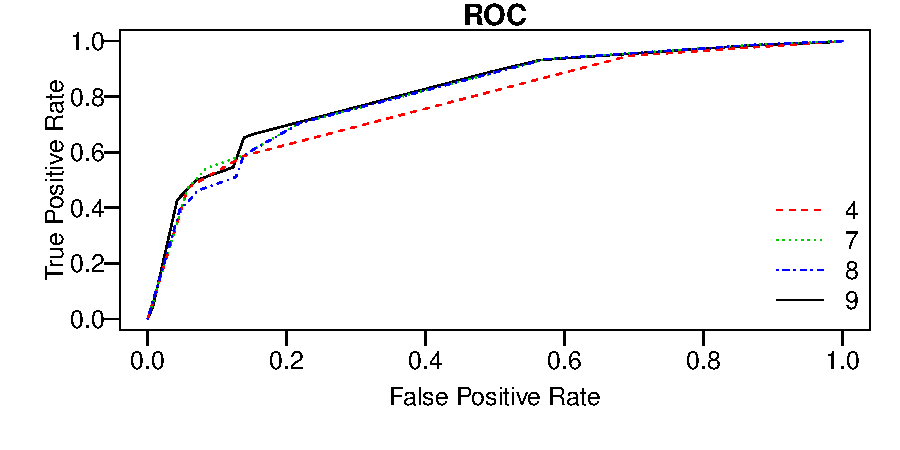
\includegraphics{HW6_DanielOsorio-020}
\end{enumerate}
\end{enumerate}
\end{enumerate}
\end{document}
